% This code is adapted from PlotNeuralNet by Haris Iqbal
% https://github.com/HarisIqbal88/PlotNeuralNet
% Used under the MIT License

\documentclass[border=8pt, multi, tikz]{standalone}
\usepackage{import}
\subimport{./layers/}{init}
\usetikzlibrary{positioning}
\usetikzlibrary{3d}
\usetikzlibrary{calc}

\def\ConvColor{rgb:green,5;red,2.5;white,5}
\def\ConvReluBNColor{rgb:green,5;red,5;white,5}
\def\CatColor{rgb:white,1;black,1}
\def\PoolColor{rgb:red,1;black,0.3}
\def\UnpoolColor{rgb:blue,2;green,1;black,0.3}
\def\FcColor{rgb:blue,5;red,2.5;white,5}
\def\FcReluColor{rgb:blue,5;red,5;white,4}
\def\SoftmaxColor{rgb:magenta,5;black,7}


\newcommand{\copymidarrow}{\tikz \draw[-Stealth,line width =0.8mm,draw={rgb:white,1;black,3}] (-0.3,0) -- ++(0.3,0);}
\renewcommand{\familydefault}{\sfdefault}

\begin{document}
\begin{tikzpicture}
\tikzstyle{connection}=[ultra thick,every node/.style={sloped,allow upside down},draw=\edgecolor,opacity=0.7]
\tikzstyle{copyconnection}=[ultra thick,every node/.style={sloped,allow upside down},draw={rgb:white,1;black,3},opacity=0.3]

\node[canvas is zy plane at x=0] (in) at (0,0,0) {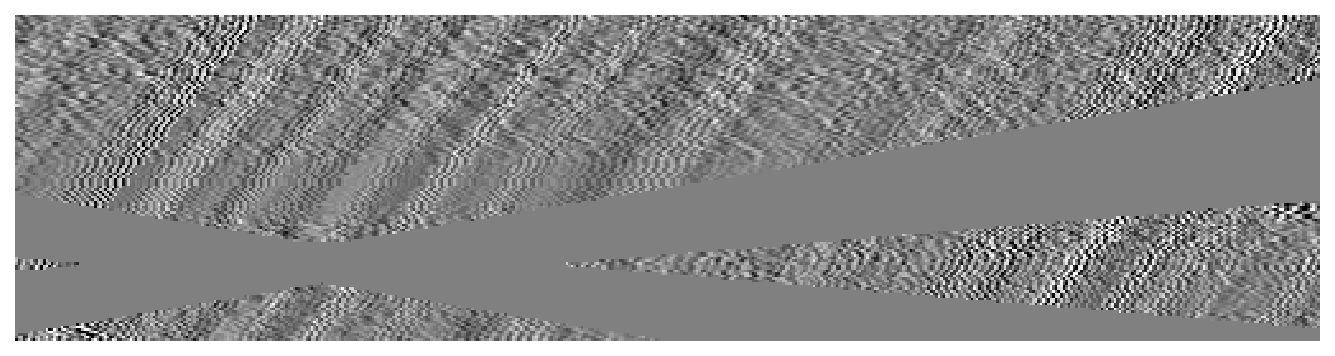
\includegraphics[width=8.1cm,height=6.5cm]{./out/figure_05_1.pdf}};
\pic[shift={(0,0,0)}] at (0,0,0) {Box={name=in,%
        fill=\ConvColor,opacity=0, height=0.75*40,width=0,depth=40}};

\pic[shift={(1,0,0)}] at (in-east) {RightBandedBox={name=cr1,%
        caption=\LARGE Down1,
        xlabel={{"32","32"}},fill=\ConvColor,bandfill=\ConvReluBNColor,%
        height=0.75*40,width={3,3},depth=40}};

\pic[shift={(0,0,0)}] at (cr1-east) {Box={name=p1,%
        fill=\PoolColor,opacity=0.5,height=0.75*32,width=1,depth=32}};


\pic[shift={(1.75,0,0)}] at (p1-east) {RightBandedBox={name=cr2,%
        caption=\LARGE Down2,
        xlabel={{"64","64"}},fill=\ConvColor,bandfill=\ConvReluBNColor,%
        height=0.75*32,width={4,4},depth=32}};

\pic[shift={(0,0,0)}] at (cr2-east) {Box={name=p2,%
        fill=\PoolColor,opacity=0.5,height=0.75*25,width=1,depth=25}};

\pic[shift={(1.5,0,0)}] at (p2-east) {RightBandedBox={name=cr3,%
        caption=\LARGE Down3,
        xlabel={{"128","128"}},fill=\ConvColor,bandfill=\ConvReluBNColor,%
        height=0.75*25,width={5,5},depth=25}};

\pic[shift={(0,0,0)}] at (cr3-east) {Box={name=p3,%
        fill=\PoolColor,opacity=0.5,height=0.75*16,width=1,depth=16}};

\pic[shift={(1.25,0,0)}] at (p3-east) {RightBandedBox={name=cr4,%
        caption=\LARGE Down4,
        xlabel={{"256","256"}},fill=\ConvColor,bandfill=\ConvReluBNColor,%
        height=0.75*16,width={6,6},depth=16}};

\pic[shift={(0,0,0)}] at (cr4-east) {Box={name=p4,%
        fill=\PoolColor,opacity=0.5,height=0.75*8,width=1,depth=8}};

\pic[shift={(1,0,0)}] at (p4-east) {RightBandedBox={name=cr5,%
        caption=\LARGE Mid,
        xlabel={{"512","512"}},fill=\ConvColor,bandfill=\ConvReluBNColor,%
        height=0.75*8,width={7,7},depth=8}};


\pic[shift={(1,0,0)}] at (cr5-east) {CatBox={name=up4,%
        xlabel={{"256",""}},fill=\UnpoolColor,bandfill=\CatColor,height=0.75*16,width=7,depth=16}};    
\pic[shift={(0,0,0)}] at (up4-east) {RightBandedBox={name=ucr4a,%
        caption=\LARGE Up4,
        xlabel={{"256","256"}},fill=\ConvColor,bandfill=\ConvReluBNColor,%
        height=0.75*16,width={6,6},depth=16}};

\pic[shift={(1.25,0,0)}] at (ucr4a-east) {CatBox={name=up3,%
        xlabel={{"128",""}},fill=\UnpoolColor,bandfill=\CatColor,height=0.75*25,width=6,depth=25}};
\pic[shift={(0,0,0)}] at (up3-east) {RightBandedBox={name=ucr3a,%
        caption=\LARGE Up3,
        xlabel={{"128","128"}},fill=\ConvColor,bandfill=\ConvReluBNColor,%
        height=0.75*25,width={5,5},depth=25}};

\pic[shift={(1.5,0,0)}] at (ucr3a-east) {CatBox={name=up2,%
        xlabel={{"64",""}},fill=\UnpoolColor,bandfill=\CatColor,height=0.75*32,width=5,depth=32}};    
\pic[shift={(0,0,0)}] at (up2-east) {RightBandedBox={name=ucr2a,%
        caption=\LARGE Up2,
        xlabel={{"64","64"}},fill=\ConvColor,bandfill=\ConvReluBNColor,%
        height=0.75*32,width={4,4},depth=32}};

\pic[shift={(2,0,0)}] at (ucr2a-east) {CatBox={name=up1,%
        xlabel={{"32",""}},fill=\UnpoolColor,bandfill=\CatColor,height=0.75*40,width=4,depth=40}};  
\pic[shift={(0,0,0)}] at (up1-east) {RightBandedBox={name=ucr1a,%
        caption=\LARGE Up1,
        xlabel={{"32","32"}},fill=\ConvColor,bandfill=\ConvReluBNColor,%
        height=0.75*40,width={3,3},depth=40}};

\pic[shift={(1,0,0)}] at (ucr1a-east) {Box={name=out,%
        xlabel="1",fill=\ConvColor,height=0.75*40,width=1,depth=40}};
\node[canvas is zy plane at x=0] (tmp) at (out-east) {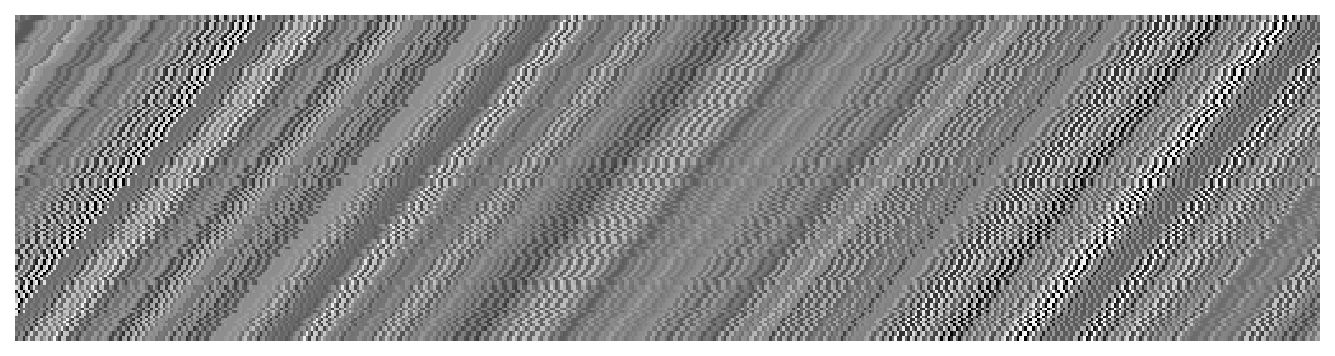
\includegraphics[width=8.1cm,height=6.5cm]{./out/figure_05_2.pdf}};

\draw [connection]  (in-east) -- node {\midarrow} (cr1-west);
\draw [connection]  (p1-east)    -- node {\midarrow} (cr2-west);
\draw [connection]  (p2-east)    -- node {\midarrow} (cr3-west);
\draw [connection]  (p3-east)    -- node {\midarrow} (cr4-west);
\draw [connection]  (p4-east)    -- node {\midarrow} (cr5-west);
\draw [connection]  (cr5-east)   -- node {\midarrow} (up4-west);
\draw [connection]  (ucr4a-east) -- node {\midarrow} (up3-west);
\draw [connection]  (ucr3a-east) -- node {\midarrow} (up2-west);
\draw [connection]  (ucr2a-east) -- node {\midarrow} (up1-west);
\draw [connection]  (ucr1a-east) -- node {\midarrow} (out-west);

\path (cr4-southeast) -- (cr4-northeast) coordinate[pos=1.25] (cr4-top) ;
\path (cr3-southeast) -- (cr3-northeast) coordinate[pos=1.25] (cr3-top) ;
\path (cr2-southeast) -- (cr2-northeast) coordinate[pos=1.25] (cr2-top) ;
\path (cr1-southeast) -- (cr1-northeast) coordinate[pos=1.25] (cr1-top) ;

\path (up4-south)  -- (up4-north)  coordinate[pos=1.25] (up4-top) ;
\path (up3-south)  -- (up3-north)  coordinate[pos=1.25] (up3-top) ;
\path (up2-south)  -- (up2-north)  coordinate[pos=1.25] (up2-top)  ;
\path (up1-south)  -- (up1-north)  coordinate[pos=1.25] (up1-top)  ;

\draw [copyconnection]  (cr4-northeast)  
-- node {\copymidarrow}(cr4-top)
-- node {\copymidarrow}(up4-top)
-- node {\copymidarrow} (up4-north);

\draw [copyconnection]  (cr3-northeast)  
-- node {\copymidarrow}(cr3-top)
-- node {\copymidarrow}(up3-top)
-- node {\copymidarrow} (up3-north);

\draw [copyconnection]  (cr2-northeast)  
-- node {\copymidarrow}(cr2-top)
-- node {\copymidarrow}(up2-top)
-- node {\copymidarrow} (up2-north);

\draw [copyconnection]  (cr1-northeast)  
-- node {\copymidarrow}(cr1-top)
-- node {\copymidarrow}(up1-top)
-- node {\copymidarrow} (up1-north);

\end{tikzpicture}
\end{document}